\chapter{Hardware Model Testing and Verification}\label{hw-model-testing}
Verification is a vital part of hardware design. For this project, all relevant functionality in the FPGA was verified by simulation.
\section{Simulation}
During FPGA development, four different testbenches were created to test the functionality of the design. The first three were module level testbenches to test the scheduler, fully-connected layer, and softmax layers. The fourth testbench tests the entire FPGA design, thus verification of the fourth testbench means that all modules are functional. Therefore, this section will discuss verification of the fourth testbench, which is a full test of the network: \texttt{neural\_net\_top\_tb.sv}, found in the directory \textit{FPGA/FPGA.srcs/sim\_1/new} of the GitHub repository as well as in Appendix \todo[inline]{appendix for testbenches}.

\subsection{Project Modifications to Simulate of the Design}
To conduct the full-scale test of the network, an input needed to be provided to the network on which to perform training. This was done by using a BRAM to store a random input generated by the same Python script (\texttt{weight\_coeff.py}) used to generate the weights for the weight BRAMS. When the simulation runs, the input to the network comes from this input BRAM rather than from the PS.

\subsection{Testing Environment}
The Vivado Simulator was used to perform simulation of the hardware. The testbench was run through Vivado's Tcl shell. During the testing process, a simulation would be ran and then diagnostic data in a test file could be  The below commands run from the Vivado Tcl show how to open the project, run the testbench for 50000 ns, and have all output written to a file.
\begin{lstlisting}
Vivado% open_proj FPGA.xpr
Scanning sources...
Finished scanning sources
open_project: Time (s): cpu = 00:00:11 ; elapsed = 00:00:13 . Memory (MB): peak = 322.016 ; gain = 71.828
Vivado% launch_simulation > sim_out
Vivado% run 50000 >> sim_out
\end{lstlisting}

\subsection{Simulation Output}
Verification and debugging was simple through the use of informative simulation output files. The project formatted signal data to be easy to read through the use of \texttt{\$display} statements. An example of this is shown in listing \ref{display-list}. This example is from \texttt{neural\_net\_top.sv} and prints the current cycle number and FC2 output and gradient data; \texttt{sf} and \texttt{sf2} are scaling factors for activations and gradients, respectively. These scaling factors allow the fixed-point Q format values to be displayed as their floating point equivalent. These types of display statements are ubiquitous in the modules of the project. Once verified, most of these display statements were commented out to prevent clutter of the simulation output file.
\begin{lstlisting}[
caption={Example debug code for simulating the functionality of the hardware model}, label={display-list}, language=SystemVerilog, upquote=true]
`ifdef DEBUG
integer clk_cycle;
integer it;

always_ff @(posedge clk) begin
  if (reset) begin
    clk_cycle   <= 0;
  end
  else begin
    clk_cycle   <=  clk_cycle + 1'b1;
  end
  $display("\n\n------ CYCLE %04d ------", clk_cycle);
  	
  $display("---FC2 GRADIENTS---");    
  $display("img_label: %d", img_label);    
  for (it = 0; it < `FC2_NEURONS; it = it + 1) begin
    $display("%02d:\t%f", it, 
      $itor($signed(fc2_gradients[it])) * sf2);
  end
  
  $display("--- FC2 OUT ---");        
  $display("fc2_buf_valid: %01b" , fc2_buf_valid);
  for (it= 0; it < `FC2_NEURONS; it=it+1) begin
    $display("%02d: %f", it, 
      $itor($signed(fc2_act_o_buf[it])) * sf); 
  end
end 
`endif    
\end{lstlisting}

With this output redirected to a text file, signal data per cycle can be easily found. Furthermore, jumping to a previous or next cycle is quick. For example, in Vim, this can be done with by pressing `N' or `n', respectively. This method of debugging with Vim is shown in Figure \ref{vim-out}, displaying the output generated from the code in Listing \ref{display-list}.
\begin{figure}
	\centering 
	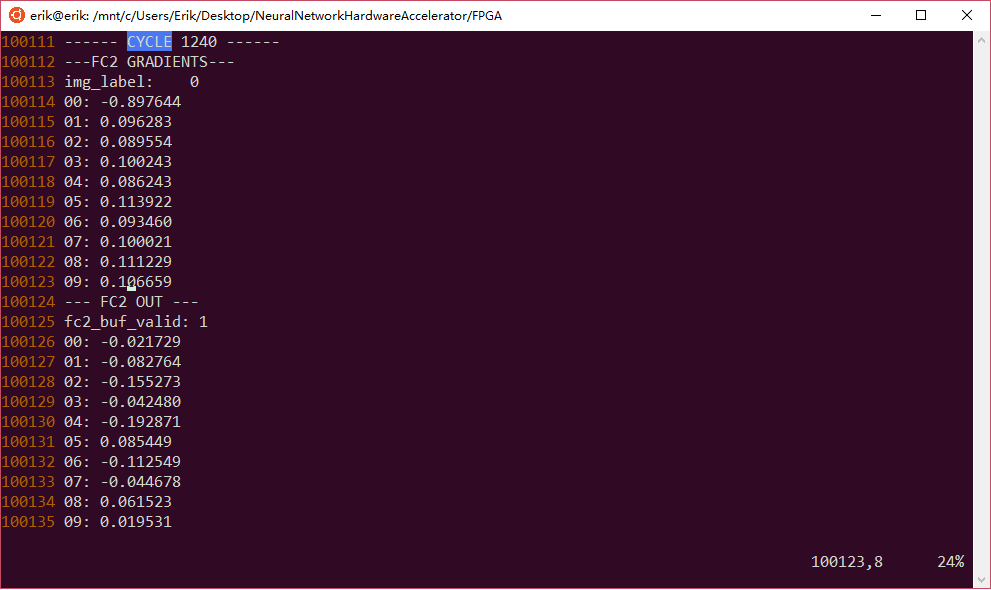
\includegraphics[width=\textwidth]{figures/vim_output}
	\caption{Jumping from cycle to cycle to view debugging data using Vim}\label{vim-out}
\end{figure}

\subsection{Correctness of Simulated Outputs}
A Python script was written to aid in verification of the hardware simulation. This script, \texttt{fpga\_forward\_backward\_pass\_test.py}, is located in Appendix \todo[inline]{appendix} as well as in the \textit{misc} folder of the project on GitHub.

This script parses the Xilinx coefficient files for the input to the network, as well as for all the neurons in all the layers and converts them to floating point numbers. The script then performs the forward pass using the parsed weights and prints the outputs. The script then computes the backward pass and also prints out all neuron and weight gradients. The hardware model can then be verified by checking that the outputs at each stage of computation align with the Python script. Note that values are not compared for equality, but for relative correctness, since the Python script uses floating point and the hardware model uses 18-bit fixed point.

Furthermore, to ensure that the script's computed outputs and gradients are correct, the script also implements gradient checking tests for itself. With this assurance,  the script's computed output and gradients were successfully verified as correct and thus could be used as a baseline against which to compare the hardware model. Note that the gradient check testing for the testing script was based on the gradient checks implemented for the software model in Chapter \ref{ch-sw-model}, and example gradient check tests are shown in Listing \ref{py-grad-check}.

\begin{lstlisting}[
caption={Gradient checks for randomly chosen weights in the Python verification script that uses inputs and weights read from the Xilinx coefficient files of the BRAMs in the hardware model. Only three non-zero gradients shown for brevity.}, label={py-grad-check}, language=SystemVerilog, upquote=true]
> python3 fpga_forward_backward_pass_test.py
../FPGA/FPGA.srcs/sources_1/ip/fc0_weights_1.17.coe
../FPGA/FPGA.srcs/sources_1/ip/fc1_weights2_1.17.coe
../FPGA/FPGA.srcs/sources_1/ip/fc2_weights_1.17.coe
Calculated gradient:    -0.003531676695546401
Numerical gradient:     -0.003531676693313557

Calculated gradient:    -0.006374946805618298
Numerical gradient:     -0.0063749433798498956

Calculated gradient:    0.0006677415295515585
Numerical gradient:     0.0006677441533042838
\end{lstlisting}

\paragraph{Forward Pass Verification}
The Python script was used to verify the correctness of the forward pass of the FPGA layer by layer. Forward pass layer outputs for softmax layer from the simulation and script are compared side-by-side in Listing \ref{sm-forward}. Since the softmax output depends on the outputs from FC0, FC1, and FC2, these layer outputs are not shown for the sake of space. From these tests, the simulated forward pass outputs of the hardware model are shown to be correct. The full outputs for every layer may be seen in the \textit{HW\_Verification} folder of the GitHub repository.

\begin{lstlisting}[
caption={Softmax output. All 10 Neuron outputs shown.}, label={sm-forward}, language=SystemVerilog, upquote=true, numbers=none]
SIMULATION                  PYTHON SCRIPT
Neuron		Activation      Neuron		Activation
00			0.102348        0			0.10235213231346099
01			0.096283        1			0.09627338472902423
02			0.089554        2			0.08953177512141873
03			0.100243        3			0.1002532810000227
04			0.086243        4			0.08622264587243636
05			0.113922        5			0.11397991662882098
06			0.093460        6			0.09343919203092571
07			0.100021        7			0.10005157131620508
08			0.111229        8			0.11123918032286678
09			0.106659        9			0.10665692066481845
\end{lstlisting}

\paragraph{Backward Pass Verification}
The backward pass was verified in the same way as the forward pass, though there are many more gradients than outputs. There is 1 gradient for each neuron and weight, totalling over 80,000 gradients. The forward pass outputs and backward pass gradients can be seen in their entirety in the \textit{hardware\_verification} folder of the GitHub repository.

The gradients in the backward pass all stem from the output layer gradients which come from the softmax function. The steps for deriving the gradients of the output layer is a softmax based neural network are explained in more detail in Chapter \ref{background}, though the gradients are essentially the softmax output visible in Listing \ref{sm-forward} except that the neuron representing the inputs class label is subtracted by 1. 

Listing \ref{rand-weight-gradients} shows randomly selected weight gradients from each of the fully-connected layers. The weight gradients depend on the neuron gradients, thus the neuron gradients for that layer must be correct for the weight gradients to be correct; because of this, only weight gradients are shown in the figure, though neuron gradients are also available for viewing in the \textit{hardware\_verification} folder. As can be seen, the gradients are calculated to relatively high accuracy. This level of accuracy is directly correlated to the fact that the gradients are all Q1.17, maximizing the amount of fractional bits. Note that the 1 integer bit is required to represent the output layer gradient (since the input class label neuron is subtracted by 1), so the radix cannot be moved any further.


\begin{lstlisting}[
caption={5 randomly selected weight gradients from each of the fully connected layers}, label={rand-weight-gradients}, language=SystemVerilog, upquote=true, numbers=none]
SIMULATION                  PYTHON SCRIPT
FC0
Neuron	Weight	Gradient	Neuron	Weight 	Gradient
09 		593 	0.000763    09   	593 	0.00076932259
19 		711 	0.006874    19 		711	 	0.00688892029
37 		412    -0.006149    37  	412    -0.00613842723
57 		128 	0.000610    57  	128 	0.00061567956
74 		485    -0.000282    74  	485    -0.00027281649

FC1
Neuron	Weight	Gradient	Neuron	Weight 	Gradient
02 		051    -0.003815    02   	051    -0.00380934976
19 		097    -0.019463    19  	097    -0.01948172921
24 		035    -0.013214    24  	035    -0.01325251269
37 		094 	0.016045    37  	094  	0.01610831241
51 		030 	0.016563    51  	030  	0.01659535729

FC2
Neuron	Weight	Gradient	Neuron	Weight 	Gradient
01  	043 	0.015907    01 		043 	0.01595727359
03  	002 	0.016861    03 		002  	0.01688975169
04  	057 	0.005745    04 		057 	0.00578264697
08  	023 	0.024437    08 		023 	0.02451471064
09  	024 	0.000542    09 		024 	0.00055094484
\end{lstlisting}
